\documentclass[margin,line]{resume}

% blue:
\definecolor{sidebarcolor}{RGB}{0, 49, 83}

\usepackage[utf8]{inputenc}
\usepackage[english,russian]{babel}
\usepackage[T1]{fontenc}
\usepackage{fontawesome}

\begin{document}

{\vspace*{-13mm}\sc \large Anton Grishin — Go Developer} \\
\begin{resume}

  \begin{minipage}[t]{0.55\textwidth}
    \section{\mysidestyle Personal\\Information}
    Moscow, Russia \\
    \faHome  \space
    \href{https://alchemmist.xyz}{\texttt{alchemmist.xyz}} \\
    \faGithub  \space
    \href{https://github.com/alchemmist/}{\texttt{alchemmist}} \\
    \faLinkedin \space
    \href{https://www.linkedin.com/in/alchemmist/}{\texttt{alchemmist}}
    \\
    \faPaperPlane \space \href{https://t.me/alchemmist}{\texttt{@alchemmist}} \\
    \faPhone \space
    \href{tel:+1234567890}{\color{blue}\texttt{+7(915)067-2638}}  \\
    \faEnvelope \space
    \href{mailto:anton.ingrish@gmail.com}{\color{blue}\texttt{anton.ingrish@gmail.com}}
  \end{minipage}

  \begin{minipage}[H]{0.18\textwidth}
    % 10.87 1.38
    \begin{textblock}{7}(10.87, 1.38)
      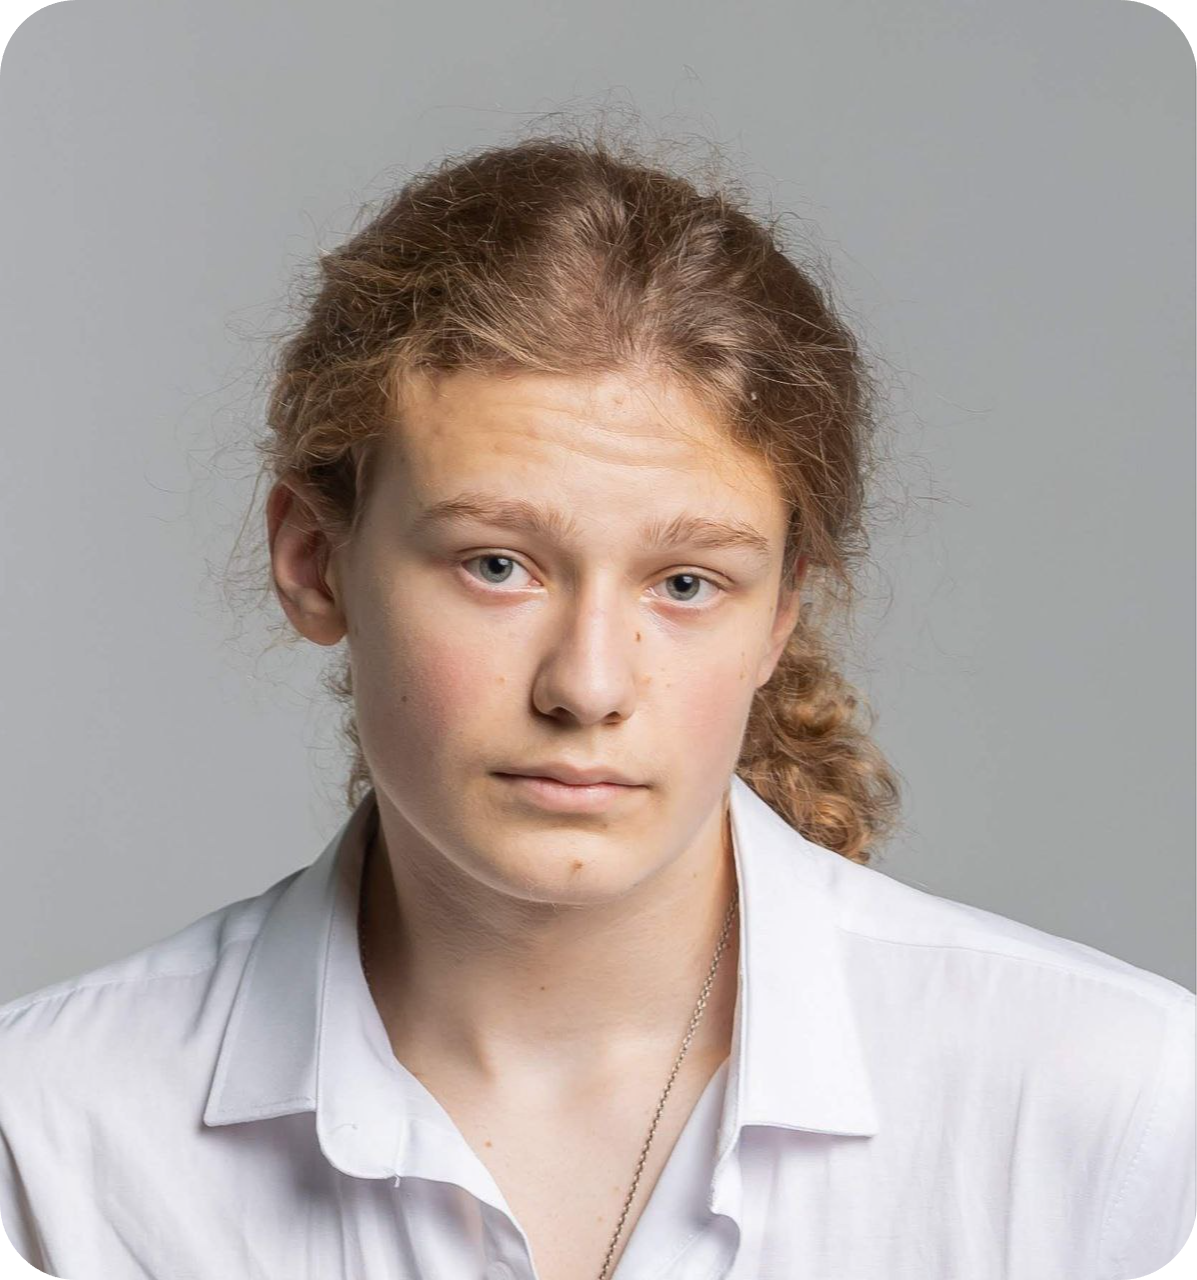
\includegraphics[width=0.270\textwidth]{../images/avatar.png}
    \end{textblock}
  \end{minipage}

  \vspace{-7mm}
  \section{\mysidestyle About Me}
  I'm a student and aspiring developer. I've been programming for 4
  years, during which I contributed to 44 repositories, made 921
  commits, and wrote 176,729 lines of code.
  I also
  \href{https://www.avito.ru/moskva/predlozheniya_uslug/prepodavatel_programmirovaniya_na_python_2556461612}{teach}
  Python and have trained over 30 students. Co-founder and developer
  at \href{https://ballkit.ru/}{Ballkit}. Former professional
  \href{https://alchemmist.github.io/CV/attachments/sport.pdf}{volleyball
  player}.

  \section{\mysidestyle Education}
  \href{https://centraluniversity.ru/}{Central University} —
  Mathematics and Computer Science, Class of 2028 \textit{(1st year)}.
  Major: Software Development. Track: Computer Science Research.
  % TODO: уточнить трек

  \section{\mysidestyle Skills}

  \vspace{0.4mm}
  \begin{description}[leftmargin=0pt, itemindent=*, itemsep=0.2pt]
    \item[Go:] \inlinecode{http}, \inlinecode{grpc},
      \inlinecode{protobuf}, \inlinecode{tgbotapi},
      \inlinecode{reflect}, \inlinecode{gofsm}.
    \item[Databases:] \inlinecode{postgres}, \inlinecode{sqlite},
      \inlinecode{redis}, \inlinecode{Yandex Object Storage}.
    \item[Message brokers:] \inlinecode{RabbitMQ}, \inlinecode{Mosquitto}.
    \item[Other technologies:] \inlinecode{SQL}, \inlinecode{Java},
      \inlinecode{JavaScript}, \inlinecode{bash}.
    \item[Dev tools:] \inlinecode{Docker}, \inlinecode{Podman},
      \inlinecode{Make}, \inlinecode{CI/CD}, \inlinecode{Linux},
      \inlinecode{Git}
  \end{description}

  \section{\mysidestyle Achievements}
  Reached the \textbf{final}
  (\href{https://alchemmist.github.io/CV/attachments/russian-chemp-final.pdf}{\texttt{1}})
  of the \href{https://events.fsp-russia.com/championship}{Russian
  Championship} in competitive programming, among 5,000 participants.
  Developed a
  \href{https://alchemmist.github.io/CV/attachments/architect.pdf}{microservice
  architecture} of 9 services for a
  \href{https://github.com/alchemmist/sportprog}{web application}
  that aggregates sports events across Russia. Also implemented an
  \href{https://github.com/alchemmist/sport-afisha/blob/main/event_parsing_service/parse_pdf.py}{algorithm}
  for parsing and verifying annual government reports on sports events.
  Tech stack: \inlinecode{Kafka}, \inlinecode{React},
  \inlinecode{RabbitMQ (FastStream)},
  \inlinecode{FastAPI},
  \inlinecode{OAuth}.

  \textbf{\href{https://alchemmist.github.io/CV/attachments/scince-for-life-win.pdf}{Winner}}
  of the scientific and practical conference
  “\href{https://conf.profil.mos.ru/academ}{Science for Life}” among
  117 projects, with a
  \href{https://github.com/smart-cab/}{smart home project} for
  private and public educational institutions.
  Tech stack: \inlinecode{Redis},
  \inlinecode{Zigbee2MQTT}, \inlinecode{websockets}, \inlinecode{Go},
  \inlinecode{Python}, \inlinecode{Flask}, \inlinecode{React}.

  \textbf{\href{https://alchemmist.github.io/CV/attachments/informatics-olimpic.pdf}{3rd
  place prize winner}} in the Moscow State Pedagogical University
  Informatics Olympiad: “Applied Informatics”

  \vspace{-2mm}
  \section{\mysidestyle Experience}\vspace{2mm}

  \begin{description}

    \item[Patch Loyalty] Loyalty program for small businesses \hfill
      \textsl{July 2024 — August 2024\vspace{1mm}}\\
      Developed a Telegram bot based on the SMB (Single Message Bot)
      model in \inlinecode{Go} for a boxed loyalty system:
      \href{https://ballkit.ru}{\texttt{ballkit.ru}}.

      \textbf{Technologies:}
      \inlinecode{Go},
      \inlinecode{tgbotapi}, \inlinecode{grpc},
      \inlinecode{gofsm}.
  \end{description}
  \vspace{-4mm}
  \section{\mysidestyle Interests}\vspace{0.7mm}

  {\textbf{Formal Verification:} I'm taking the course
    \texttt{\href{https://softwarefoundations.cis.upenn.edu}{softwarefoundations}}.
    Finished the first volume and
    \href{https://github.com/alchemmist/coq-learning}{proved} 250
  theorems in \inlinecode{Coq}.} \\

  \vspace{-6mm}

  \textbf{Linux:} I use Arch with the Hyprland compositor. Published my
  \href{https:/github.com/alchemmist/.dotfiles}{\texttt{.dotfiles}}.
  Built my Neovim
  \href{https://github.com/alchemmist/.dotfiles/tree/main/nvim}{configuration}
  and
  \href{https://github.com/alchemmist/nothing.nvim}{colorscheme} from scratch.
  Wrote more than 20 custom
  \href{https://github.com/alchemmist/.dotfiles/tree/main/scripts}{scripts}.

\end{resume}

\begin{minipage}[H]{9.18\textwidth}
  \begin{textblock}{7}(-0.65, 15.1)
    \begingroup
    \hspace{35mm}
    \hypersetup{urlcolor=gray!90}
    \large
    \href{https://github.com/alchemmist}{→ more projects on
    \underline{GitHub}}
    \endgroup
  \end{textblock}

\end{minipage}

\clearpage

\end{document}
